\documentclass[border=6pt]{standalone}
\usepackage{tikz}
\usetikzlibrary{arrows.meta, positioning, calc}

% Palette presentation
\definecolor{surplus}{HTML}{27AE60}
\definecolor{deficit}{HTML}{C0392B}
\definecolor{depot}{HTML}{2980B9}
\definecolor{accent}{HTML}{F39C12}
\definecolor{tdark}{HTML}{23373B}

\begin{document}
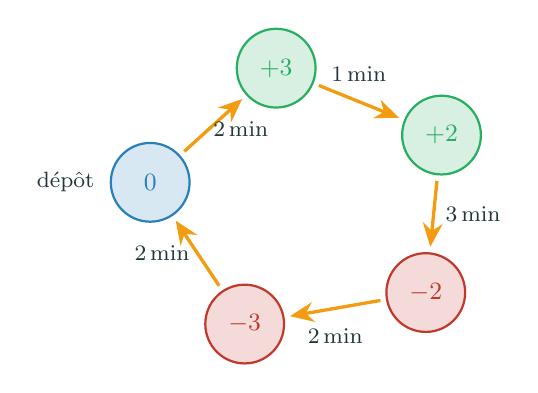
\begin{tikzpicture}[
    >={Stealth[length=3mm, width=2.5mm]},
    station/.style={
      circle, draw, thick, minimum size=1.0cm, inner sep=0pt,
      font=\small\bfseries, text=tdark
    },
    depotnode/.style={station, draw=depot, fill=depot!18, text=depot},
    surplusnode/.style={station, draw=surplus, fill=surplus!18, text=surplus},
    deficitnode/.style={station, draw=deficit, fill=deficit!18, text=deficit},
    arc/.style={
      ->, very thick, accent,
      shorten >=2pt, shorten <=2pt
    },
    lbl/.style={font=\footnotesize, text=tdark}
  ]

  % Sommets
  \node[depotnode]    (d)  at (0,    0)      {$0$};
  \node[surplusnode]  (s1) at (1.6,  1.45)   {$+3$};
  \node[surplusnode]  (s2) at (3.7,  0.6)    {$+2$};
  \node[deficitnode]  (s3) at (3.5, -1.4)    {$-2$};
  \node[deficitnode]  (s4) at (1.2, -1.8)    {$-3$};

  % Etiquette depot (a gauche pour ne pas chevaucher l'arc sortant)
  \node[lbl, left=2pt of d]  {dépôt};

  % Arcs du cycle
  \draw[arc] (d)  -- (s1);
  \draw[arc] (s1) -- (s2);
  \draw[arc] (s2) -- (s3);
  \draw[arc] (s3) -- (s4);
  \draw[arc] (s4) -- (d);

  % Poids c_ij = temps de trajet (au milieu de chaque arc, decale vers l'exterieur)
  \node[lbl] at ($(d)!0.5!(s1)  + ( 0.35,-0.05)$) {$2$\,min};
  \node[lbl] at ($(s1)!0.5!(s2) + ( 0.00, 0.35)$) {$1$\,min};
  \node[lbl] at ($(s2)!0.5!(s3) + ( 0.50, 0.00)$) {$3$\,min};
  \node[lbl] at ($(s3)!0.5!(s4) + ( 0.00,-0.35)$) {$2$\,min};
  \node[lbl] at ($(s4)!0.5!(d)  + (-0.45, 0.00)$) {$2$\,min};

\end{tikzpicture}
\end{document}
